\section{Navigation Outcomes, Runtime Checks, and Additional Cases}
\label{app:navigation}

Which aspects of navigation change together? The full metric run contains
99 paired episode IDs across KuJiaLe scenes 0031, 0036, and 0066, with 33
per scene. Original and converted runs share instructions, start states,
episode definitions, and agent settings. Table~\ref{tab:app-navfull} adds
oracle success and paired intervals to the main results.

\begin{table}[htbp]
\centering\small
\setlength{\tabcolsep}{4pt}
% Generated by appendix/build_tables.py; source hashes in table_sources.json.
\begin{tabular}{lrrrr}
\toprule
Metric & Original & Converted & $\Delta$ & 95\% paired CI \\
\midrule
SR (\%) & 52.530 & 48.480 & -4.040 & [-15.150, 7.070] \\
SPL (\%) & 47.390 & 42.980 & -4.410 & [-14.170, 5.140] \\
Oracle success (\%) & 66.670 & 61.620 & -5.050 & [-15.150, 5.050] \\
Navigation error & 3.680 & 3.631 & -0.049 & [-0.646, 0.539] \\
Trajectory length & 6.975 & 7.060 & +0.084 & [-0.737, 0.930] \\
Action steps & 233.647 & 275.394 & +41.748 & --- \\
Fall rate & 0.020 & 0.020 & +0.000 & --- \\
Stuck rate & 0.000 & 0.000 & +0.000 & --- \\
\bottomrule
\end{tabular}

\caption{Navigation metrics over all 99 episode pairs. Differences are
Converted minus Original. SR, SPL, and oracle success use percentages;
NE and TL retain the evaluator's distance units. Intervals are the recorded
95\% paired bootstrap intervals; dashes denote metrics without a retained
interval. Fall rate (FR) and stuck rate (StR) are fractions of episodes
with the corresponding recorded failure reason.}
\label{tab:app-navfull}
\end{table}

SR records completion under the evaluator's success rule. NE is the final goal
distance, TL is executed path length, and SPL weights success by path efficiency,
$S L^*/\max(L,L^*)$, where $L^*$ is reference path length. Oracle success
records whether the episode reaches the success region along its path. SR and
SPL decrease in aggregate, while mean NE decreases slightly and TL increases.
The measures therefore capture different properties of the executed episodes.
The paired intervals span zero; the 17 success-to-failure and 13
failure-to-success transitions describe the observed redistribution directly.

Each episode has one metric rollout per material condition. The observed
turnover includes any runtime variability, for which these runs provide no
same-condition repeat estimate. Grounding and navigation use different scenes
and models, so they provide complementary observations rather than a measured
causal chain from a particular pointing error to an episode outcome.

\subsection{Loading and rendering the scenes}
Separate fresh-launch checks exercise each of the three scenes three times
per condition, totaling 18 launches. All complete successfully
(Table~\ref{tab:app-navload}). Ready time and warm-up frame rate are similar
at this scale. These measurements concern initialization and rendering; they
are distinct from the 198 navigation rollouts.

\begin{table}[htbp]
\centering\small
\setlength{\tabcolsep}{3pt}
% Generated by appendix/build_tables.py; source hashes in table_sources.json.
\begin{tabular}{lrrrr}
\toprule
Condition & Loads & Ready time (s) & Warm-up FPS & GPU memory (MB) \\
\midrule
Original & 9/9 & 13.95 [11.64, 16.28] & 2.36 [2.01, 2.70] & 3807 [3748, 3862] \\
Converted & 9/9 & 14.12 [12.31, 16.24] & 2.42 [2.08, 2.73] & 3829 [3689, 3971] \\
\bottomrule
\end{tabular}

\caption{Fresh-launch scene checks. Each condition has nine successful loads
across three scenes. Values reproduce the recorded mean and interval summaries
for ready time, warm-up frame rate, and GPU memory (bootstrap 95\% CIs).}
\label{tab:app-navload}
\end{table}

\subsection{Twelve paired recorded examples}
The following panels show selected episode reruns from all three scenes,
including asymmetric outcomes, divergent routes with the same binary outcome,
and similar-route examples. Each episode retains original and converted
start, middle, and ending frames with path overlays. This temporal context
shows how a final observation relates to the route that preceded it.

In episode 898, the converted route loops near the starting room while the
original route extends farther through the interior. Episode 891 shows a
wider converted detour, whereas episode 598 reaches similar kitchen views
in both recordings. These examples make the variety of paired trajectory
changes visible beyond the final success indicator.

The full 99-pair metric runs were video-free. These recorded reruns share
episode IDs with that evaluation but have their own trajectories and outcomes;
the figures do not substitute rerun scores for the full-run measurements.
Keeping both conditions visible also avoids treating a changed path as
necessarily a changed success status.

\begin{figure}[htbp]
\centering
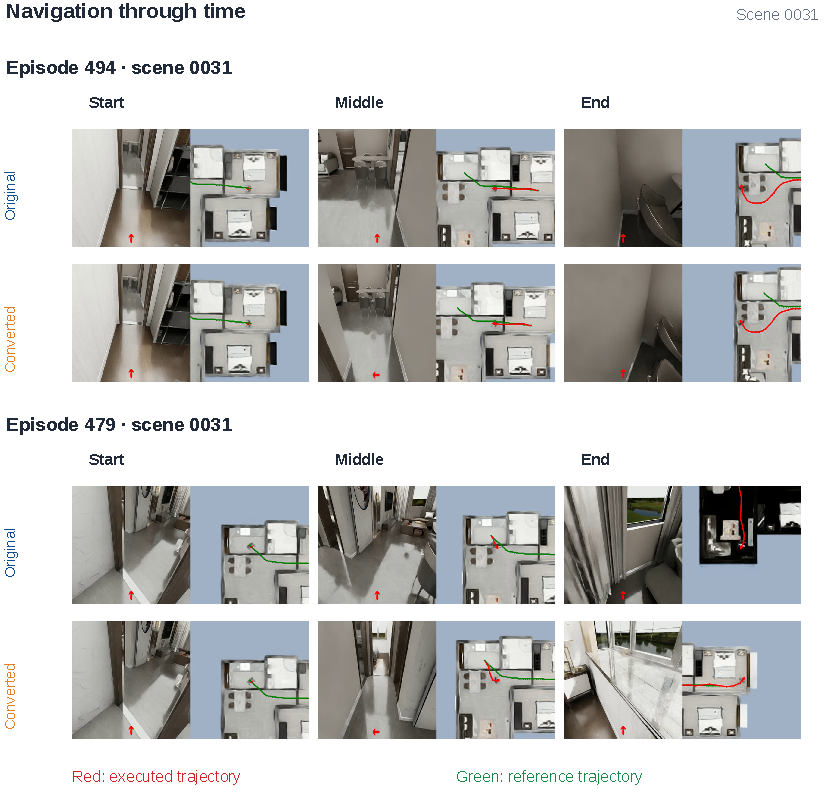
\includegraphics[width=\linewidth,height=.84\textheight,keepaspectratio]{appendix_navigation_cases_01.pdf}
\caption{Paired navigation reruns: episodes 494 and 479 in scene 0031. Rows show Original and Converted; columns show the start, middle, and end. Red maps the executed path and green the reference path. These recordings are separate from the 99-pair metric runs.}
\label{fig:app-navcases1}
\end{figure}

\begin{figure}[p]
\centering
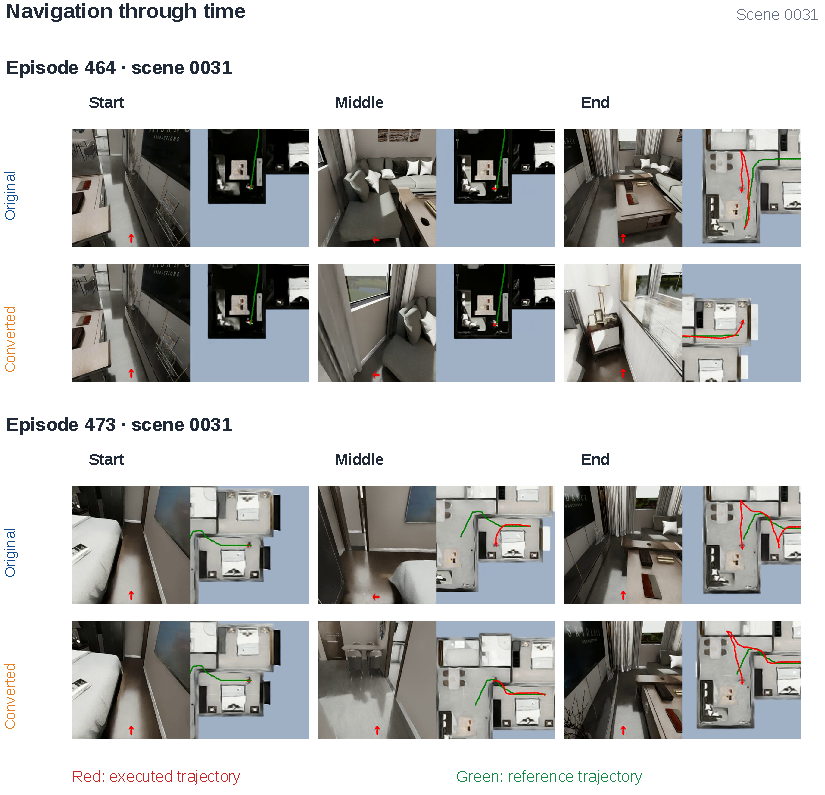
\includegraphics[width=\linewidth,height=.84\textheight,keepaspectratio]{appendix_navigation_cases_02.pdf}
\caption{Paired navigation reruns: episodes 464 and 473 in scene 0031. Rows show Original and Converted; columns show the start, middle, and end. Red maps the executed path and green the reference path. These recordings are separate from the 99-pair metric runs.}
\label{fig:app-navcases2}
\end{figure}

\begin{figure}[p]
\centering
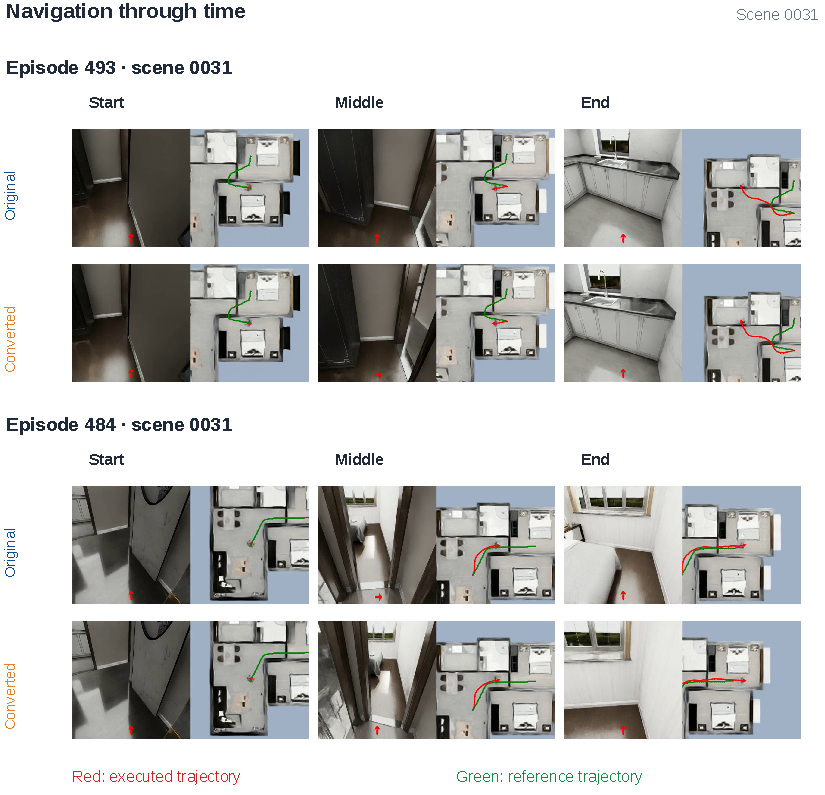
\includegraphics[width=\linewidth,height=.84\textheight,keepaspectratio]{appendix_navigation_cases_03.pdf}
\caption{Paired navigation reruns: episodes 493 and 484 in scene 0031. Rows show Original and Converted; columns show the start, middle, and end. Red maps the executed path and green the reference path. These recordings are separate from the 99-pair metric runs.}
\label{fig:app-navcases3}
\end{figure}

\begin{figure}[p]
\centering
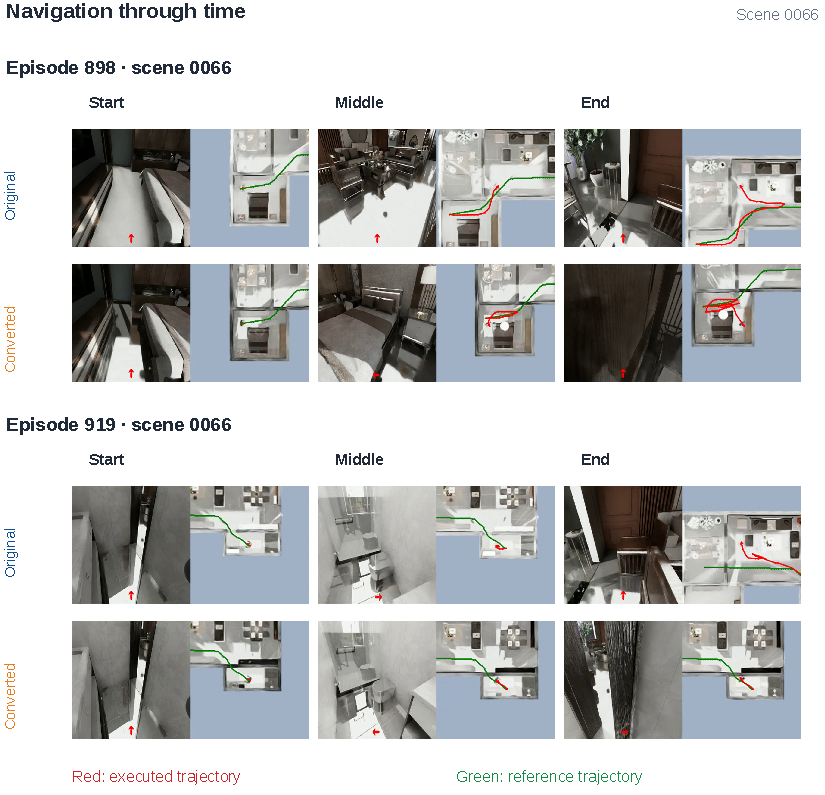
\includegraphics[width=\linewidth,height=.84\textheight,keepaspectratio]{appendix_navigation_cases_04.pdf}
\caption{Paired navigation reruns: episodes 898 and 919 in scene 0066. Rows show Original and Converted; columns show the start, middle, and end. Red maps the executed path and green the reference path. These recordings are separate from the 99-pair metric runs.}
\label{fig:app-navcases4}
\end{figure}

\begin{figure}[p]
\centering
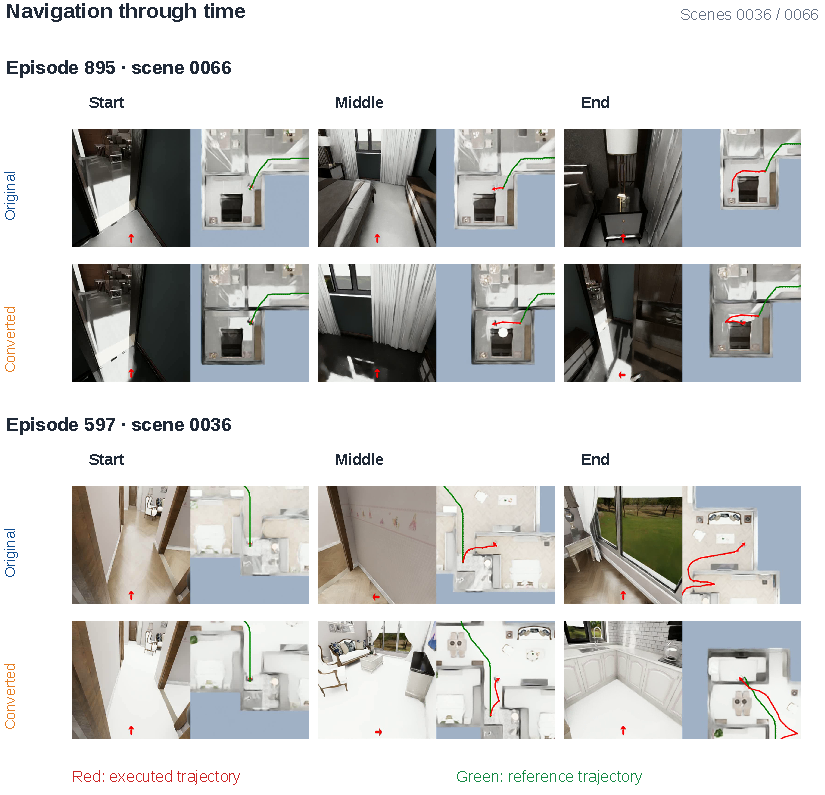
\includegraphics[width=\linewidth,height=.84\textheight,keepaspectratio]{appendix_navigation_cases_05.pdf}
\caption{Paired navigation reruns: episodes 895 (scene 0066) and 597 (scene 0036). Rows show Original and Converted; columns show the start, middle, and end. Red maps the executed path and green the reference path. These recordings are separate from the 99-pair metric runs.}
\label{fig:app-navcases5}
\end{figure}

\begin{figure}[p]
\centering
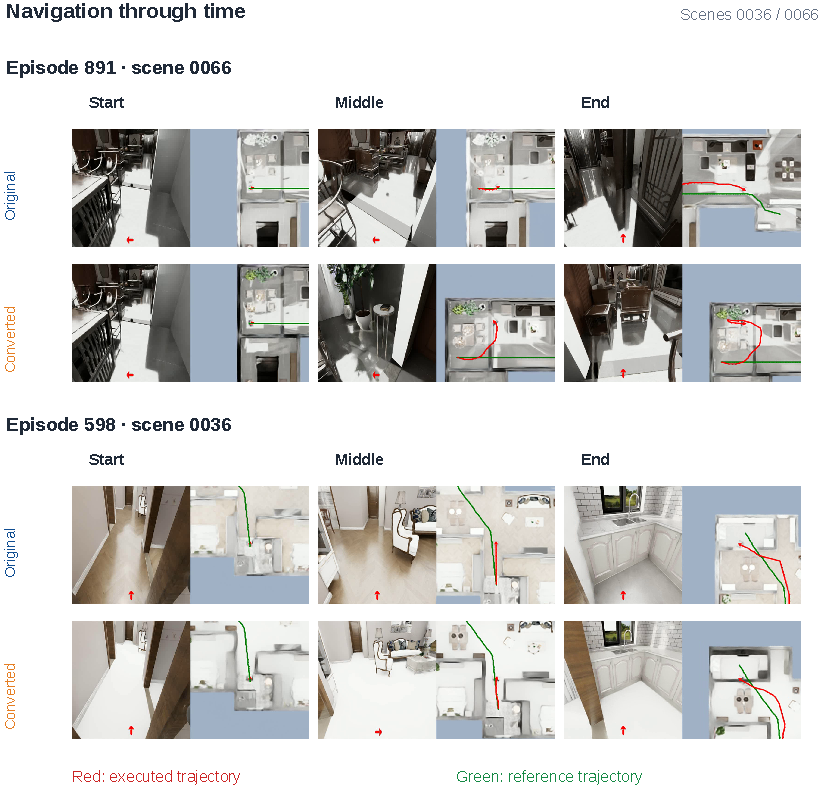
\includegraphics[width=\linewidth,height=.84\textheight,keepaspectratio]{appendix_navigation_cases_06.pdf}
\caption{Paired navigation reruns: episodes 891 (scene 0066) and 598 (scene 0036). Rows show Original and Converted; columns show the start, middle, and end. Red maps the executed path and green the reference path. These recordings are separate from the 99-pair metric runs.}
\label{fig:app-navcases6}
\end{figure}
\FloatBarrier
